%%%% Document type  %%%%
\documentclass[preprint,12pt,fleqn]{article}
 \usepackage{ragged2e}
\usepackage{authblk}  % Package for author affiliations
% \usepackage{nopageno} % no page numbers
\usepackage[rightcaption]{sidecap}
\usepackage{placeins} % Floatbarrier



\usepackage{amsmath}
\usepackage{graphicx}
\usepackage{enumitem}
\usepackage{booktabs}


\usepackage[most]{tcolorbox}
\newtcolorbox[auto counter,number within=chapter]{definition}[1][]{
  enhanced,
  breakable,
  fonttitle=\scshape,
  title={Definition \thetcbcounter},
  #1
}

%%%% Document structure %%%%
%\usepackage{geometry}
\usepackage[verbose=true,letterpaper]{geometry}
\geometry{
%    a4paper,
%    left=30mm,
%    right=30mm,
%    top=30mm,
%    bottom=30mm,
    textheight=9in,
    textwidth=6in,
    top=1in,
    headheight=12pt,
    headsep=25pt,
    footskip=30pt,
   % phone  
   %a5paper,
   %width=120mm,
  %height=180mm,
}

\usepackage{lineno} % used along with \linenumbers after begin document. 
\usepackage{setspace} 
\setstretch{1.2}
\makeatletter % The following lines get rid of footer stating pre-preint to elsevier.
\def\ps@pprintTitle{%
\let\@oddhead\@empty
\let\@evenhead\@empty
\def\@oddfoot{}%
\let\@evenfoot\@oddfoot}
\makeatother
\graphicspath{ {../images/} }
\usepackage{pgf} % calculate cohort stats percentage

%%%% Bibliography   %%%%
\usepackage{natbib}
\setcitestyle{numbers,sort&compress}
\setcitestyle{sort&compress}
\usepackage{hypernat} 
    
%%%% Aesthetics     %%%%
\usepackage{microtype}
% \RequirePackage{times} % Font
\usepackage{ccaption}
\usepackage{siunitx}
\usepackage[T1]{fontenc}
\usepackage[utf8]{inputenc}
\usepackage{nameref}% this allows a reference be named, to print unnumbered references by their section name (used here for linking to Supplemental text in this case).

%%%% Paragraph Formatting %%%
\setlength{\parindent}{2em}
\setlength{\parskip}{6pt plus 2pt minus 1pt}

%%%% Supplemental labels%%%%
%Define command to start a supplemental section
%set the supplemental letter used for figures (e.g. Figure E1)
\newcommand{\beginsupplement}{%
        \setcounter{table}{0}
        \renewcommand{\thetable}{E\arabic{table}}%
        \setcounter{figure}{0}
        \renewcommand{\thefigure}{E\arabic{figure}}%
         }

%%%% Building tables%%%%
\usepackage{booktabs} % required for tables
\usepackage{rotating,tabularx} 
\newcolumntype{Z}{ >{\centering\arraybackslash}X } % defining table content layout per box
\usepackage{ltablex} % allow page break between lines in tabularx
% \usepackage{caption} \captionsetup{font=normalsize} % to set the caption size as normal even when table is tiny.
\usepackage{multirow}
\usepackage{pdflscape}

%%%% Colors %%%%
\usepackage{xcolor} 
\definecolor{natureblue}{RGB}{5,110,210}
    \usepackage[colorlinks]{hyperref} 
\AtBeginDocument{%this allows colours to chage from the defined elsearticle template.
\hypersetup{
    	colorlinks=true,
        linkcolor={natureblue},
    	citecolor={natureblue},
        filecolor=blue!50!black,
        urlcolor=cyan,
    	}}

\definecolor{kispiblack}{HTML}{333333}
\definecolor{kispidarkblue}{HTML}{023047}
\definecolor{kispidarkgreen}{HTML}{006666}
\definecolor{kispired}{HTML}{C70000}
\definecolor{kispilink}{HTML}{007DB8}%219EBC
% \color{kispi_black} %default
\definecolor{kispiblue}{HTML}{701A57}
% City sunset: https://www.color-hex.com/color-palette/40131
\definecolor{colorSUNSET1}{HTML}{eeaf61}
\definecolor{colorSUNSET2}{HTML}{fb9062}
\definecolor{colorSUNSET3}{HTML}{ee5d6c}
\definecolor{colorSUNSET4}{HTML}{ce4993}
\definecolor{colorSUNSET5}{HTML}{6a0d83}
\definecolor{natureblue}{RGB}{5,110,210}    
\usepackage{dirtree}  % Load the dirtree package

% command to use these colors and formatting; xspace for correct spacing including with punctuation marks.
\usepackage{xspace}
\newcommand{\variablesdarkgreen}[1]{\textbf{\textcolor{kispidarkgreen}{#1}}\xspace}

%%%% Fancy stuff %%%%
%\usepackage{fancyhdr}
%\pagestyle{fancy}
%\lhead{My Name}
%\chead{}
%\rhead{\thepage}
%\cfoot{} % get rid of the page number 
%\renewcommand{\headrulewidth}{0pt}
%\renewcommand{\footrulewidth}{0pt}
 
 
%\usepackage{fancyhdr}
%\usepackage{lastpage}
%\pagestyle{fancy}
%\fancyhf{}
%\rfoot{\thepage}
%\cfoot{} % get rid of the page number 
%\renewcommand{\headrulewidth}{0pt}
%\renewcommand{\footrulewidth}{0pt}

 
\usepackage{tocloft}  % Customizing the Table of Contents
\setcounter{tocdepth}{2}


%%%% Include code %%%%
% \usepackage{verbatim}

\usepackage{listings}
\lstset{
    basicstyle=\ttfamily\small,
    breaklines=true,
    postbreak=\mbox{\textcolor{red}{$\hookrightarrow$}\space}, % 
    breakatwhitespace=false,
    % frame=single,
    showstringspaces=TRUE, % Don't show spaces in strings as special characters
    tabsize=2, 
    language=sh 
}

\usepackage{fontspec}
% \setmainfont{IBM Plex Sans}
% \setmonofont{IBM Plex Mono}
% \usepackage{unicode-math}
% \setmathfont{IBM Plex Math}

%\renewcommand{\rmdefault}{ptm}
%\renewcommand{\sfdefault}{phv}


% {{\ttfamily \hyphenchar\the\font=`\-} % set hyphenation for texttt blocks

\usepackage{xpatch}
\xpatchcmd{\AC@deflist}
  {\addtolength{\leftmargin}{\labelsep}}
  {\addtolength{\leftmargin}{\labelsep}\setlength{\itemsep}{0pt}}
  {}{}
\makeatother
\usepackage[printonlyused,withpage,nohyperlinks]{acronym}
\begin{document}
\newcounter{myboxcounter}
\newcommand{\boxlabel}[1]{%
  \refstepcounter{myboxcounter}%
  \label{#1}%
}

\title{An Actor-Critic Reinforcement Learning Framework for Genetic Variant Pathogenicity}

\author[1]{Dylan Lawless\thanks{Addresses for correspondence: \href{mailto:Dylan.Lawless@uzh.ch}{Dylan.Lawless@uzh.ch}}}
\affil[1]{Department of Intensive Care and Neonatology, University Children's Hospital Zürich, University of Zürich, Switzerland.}

\maketitle
\justify
% \tableofcontents
% \listoffigures
% \listoftables

\section*{Acronyms}
\renewenvironment{description} % Internally acronym uses description which we redefine to make condense spacing. 
{\list{}{\labelwidth0pt\itemindent-\leftmargin
    \parsep-1em\itemsep0pt\let\makelabel\descriptionlabel}}
               {\endlist}
\begin{acronym} 
 \acro{acat}[ACAT]{Aggregated Cauchy Association Test }
 \acro{acmg}[ACMG]{American College of Medical Genetics and Genomics}
 \acro{af}[AF]{Allele Frequency}
 \acro{ad}[AD]{Autosomal Dominant}
 \acro{ar}[AR]{Autosomal Recessive}
 \acro{gwas}[GWAS]{Genome Wide Association Test}
 \acro{maf}[MAF]{Minor Allele Frequency}
 \acro{prs}[PRS]{Polygenic Risk Score} 
 \acro{qc}[QC]{Quality Control}
 \acro{qv}[QV]{Qualifying variant}
 \acro{rdf}[RDF]{Resource Description Framework}
 \acro{ax}[QV\textsubscript{ax}]{Axiomatic Variants}
 \acro{sf}[SF]{Secondary Findings}
 \acro{skat}[SKAT]{sequence kernel association test} 
 \acro{sphn}[SPHN]{Swiss Personalized Health Network}
 \acro{vqsr}[VQSR]{Variant Quality Score Recalibration}
 \acro{vsat}[VSAT]{Variant Set Association Test}
 \acro{wgs}[WGS]{Whole Genome Sequencing}
\end{acronym}
 
\section*{Abstract}
We present a reinforcement learning (RL) framework designed to predict genetic variant pathogenicity by integrating established metrics such as the American College of Medical Genetics and Genomics (ACMG) score, gene risk factors, and population frequency. Using simulated genetic data with realistic variability and label noise, we systematically evaluated RL performance across multiple scenarios, employing metrics including ROC curves, AUC, calibration plots, and learning dynamics. Results indicate robust predictive accuracy and effective learning, demonstrating RL’s potential as a practical tool for genomic variant interpretation, setting the stage for integration into a broader Bayesian classification framework.

\section{Introduction}
Precise interpretation of genetic variants remains a central challenge in precision medicine, significantly impacting clinical decision-making and patient care. Differentiating pathogenic from benign variants accurately is essential for genetic diagnostics. Standard classification methods often face limitations due to incomplete or uncertain annotations, motivating the exploration of adaptive machine learning techniques.

Reinforcement learning (RL) provides an appealing alternative to traditional supervised methods by utilising evaluative rather than instructive feedback. Instead of explicitly labelled outcomes, RL algorithms receive scalar rewards reflecting decision quality, thereby naturally balancing exploration of uncertain genomic space and exploitation of known information. Inspired by the classical $k$-armed bandit problem, our approach adapts an actor-critic algorithm to genomic data, using key features already available clinically—such as the GuRu score, gene risk categorisation, and population allele frequency—to classify variant pathogenicity.

In this study, we systematically quantify RL performance using a comprehensive suite of evaluation metrics within simulated genomic scenarios, incorporating realistic data imperfections. Our goal is to identify RL methodologies and parameter configurations that exhibit robust and accurate predictive capabilities, thus laying the groundwork for subsequent integration into a Bayesian analytical framework aimed at interpreting genetic evidence in clinical diagnostics.


% \section{Introduction}
%The precise interpretation of genetic variants is a crucial challenge in the era of personalised medicine. In particular, it is of great clinical importance to accurately distinguish between pathogenic and benign variants. In this study, we propose a reinforcement learning (RL) framework that utilises the American College of Medical Genetics and Genomics (ACMG) score, together with other key features such as gene number and population frequency, to predict the pathogenicity of genetic variants. Our approach is designed to learn from a training dataset comprising variants with known disease-causing status and to extend this learning to classify variants of unknown pathogenicity.
%
%Reinforcement learning differs markedly from traditional supervised methods in that it relies on evaluative feedback rather than instructive labels. Instead of being provided with the correct outcome for each input, the RL agent receives a scalar reward that reflects the quality of its decision. This evaluative feedback necessitates an explicit exploration of the input space in order to strike a balance between exploiting known information and exploring uncertain regions. Our study leverages this property by using known disease-causing variants to guide the learning process, thereby enabling the prediction of pathogenicity in previously unlabelled cases.
%
%The theoretical inspiration for our methodology is drawn from the classic $k$-armed bandit problem, where an agent must repeatedly choose from a set of actions, each associated with an uncertain reward distribution. By adapting an actor-critic algorithm to this genomic context, our method aims to derive an optimal policy that effectively uses the GuRu score and related features to classify variants. The performance of the model is rigorously evaluated through multiple metrics, including receiver operating characteristic (ROC) curves, the area under the ROC curve (AUC), precision, recall, F1 score, cumulative learning curves, and calibration plots. These evaluation tools provide a comprehensive assessment of both the convergence behaviour and the predictive accuracy of the proposed approach.

\section{Methods}
Our investigation employs a synthetic dataset designed to mimic the characteristics of genetic variant data. The dataset comprises 10,000 variants, with 50\% of the entries containing known pathogenicity labels and the remaining 50\% left unlabelled for prediction purposes. Variants are generated to reflect realistic genomic scenarios by incorporating features such as the GuRu score, gene number, and population frequency. Notably, variants occurring in genes numbered 4 to 10 are considered to be of higher risk, while those in genes 1 to 6 are deemed to be of lower risk. Furthermore, to replicate potential misannotations in empirical data, a proportion of the known labels is deliberately flipped according to a predefined noise parameter.

The reinforcement learning framework is implemented via an actor-critic algorithm. In our formulation, the state space is constructed by discretising the GuRu score into four bins, the population frequency into three bins, and the gene risk into a binary indicator; the product of these discretisations yields 24 unique states. The action space is binary, corresponding to the two possible classifications: benign (0) or pathogenic (1). At each iteration, the RL agent observes a state corresponding to a variant and selects an action using a probabilistic policy derived from a sigmoid function applied to a vector of actor weights. A reward of +1 is granted if the predicted label matches the true pathogenicity, otherwise a penalty of -1 is imposed. The temporal-difference (TD) error, defined as the difference between the received reward and the critic’s estimate of the state value, is used to update both the actor and critic weights using learning rates $\alpha$ and $\beta$, respectively.

In order to assess the robustness of our model, we vary three critical parameters: the noise level in the training labels, the actor learning rate, and the critic learning rate. For each combination of these parameters, the model is trained for 20 epochs and a variety of performance metrics are recorded. The evaluation comprises epoch-level measures of average TD error and average reward, as well as more detailed assessments including ROC curves with associated AUC values, precision, recall, F1 scores, cumulative learning curves and calibration plots. All these metrics are aggregated and visualised using faceted plots, thus allowing for a comprehensive comparison of the effects of different parameter settings.

The complete experimental implementation is written in R. Synthetic data are generated according to the specified stratification and noise levels, and the RL model is trained on a randomly partitioned training set for each combination of parameters. Performance on a held-out test set is evaluated and visualised through several plots, each of which is saved as an individual PNG file for further examination.

\section{Results}

In this study, we evaluated the performance of a reinforcement learning model that leverages GuRu scores and additional variant features to predict pathogenicity in genetic data. The model was trained on known disease‐causing variants and subsequently applied to predict the status of unknown variants. The experiments varied the noise level in the training labels, as well as the actor ($\alpha$) and critic ($\beta$) learning rates. Performance was assessed using several metrics: average reward and temporal-difference (TD) error during training, cumulative learning curves, receiver operating characteristic (ROC) curves with the corresponding area under the curve (AUC), and calibration of predicted probabilities.

Figure~\ref{fig:epoch_reward} shows the evolution of the average reward per epoch during training. This plot demonstrates that, under different parameter settings and noise levels, the model progressively improves its reward performance over successive epochs, indicating effective learning.

Complementing this, Figure~\ref{fig:epoch_td} presents the average TD error per epoch. The decreasing TD error over time reflects the convergence of the model’s value estimates and confirms that the learning algorithm is stabilising across training epochs.

Figure~\ref{fig:learning} depicts the cumulative average reward over training samples, providing a continuous view of the learning progress. The gradual increase in the cumulative reward further supports the model's ability to optimise its decision-making process over time.

For evaluating the classification performance, Figure~\ref{fig:roc_curve} displays the ROC curves for various parameter combinations. These curves illustrate the trade-off between the true positive rate and the false positive rate, with several settings yielding high discrimination ability. This observation is reinforced by the AUC heatmap in Figure~\ref{fig:auc}, which summarises how AUC values vary as a function of $\alpha$ and $\beta$ for each noise level. In some cases, AUC values exceed 0.8, demonstrating robust performance.

Finally, Figure~\ref{fig:calibration} provides a calibration plot comparing the mean predicted probabilities to the observed proportions of pathogenic variants. The close alignment between the predicted and observed values across different parameter settings indicates that the model’s probability estimates are well-calibrated.

Overall, these results demonstrate that our reinforcement learning framework is capable of effectively learning to predict variant pathogenicity from noisy data, with the performance being sensitive to the learning rate parameters and the level of label noise.

\begin{figure}[h]
    \centering
    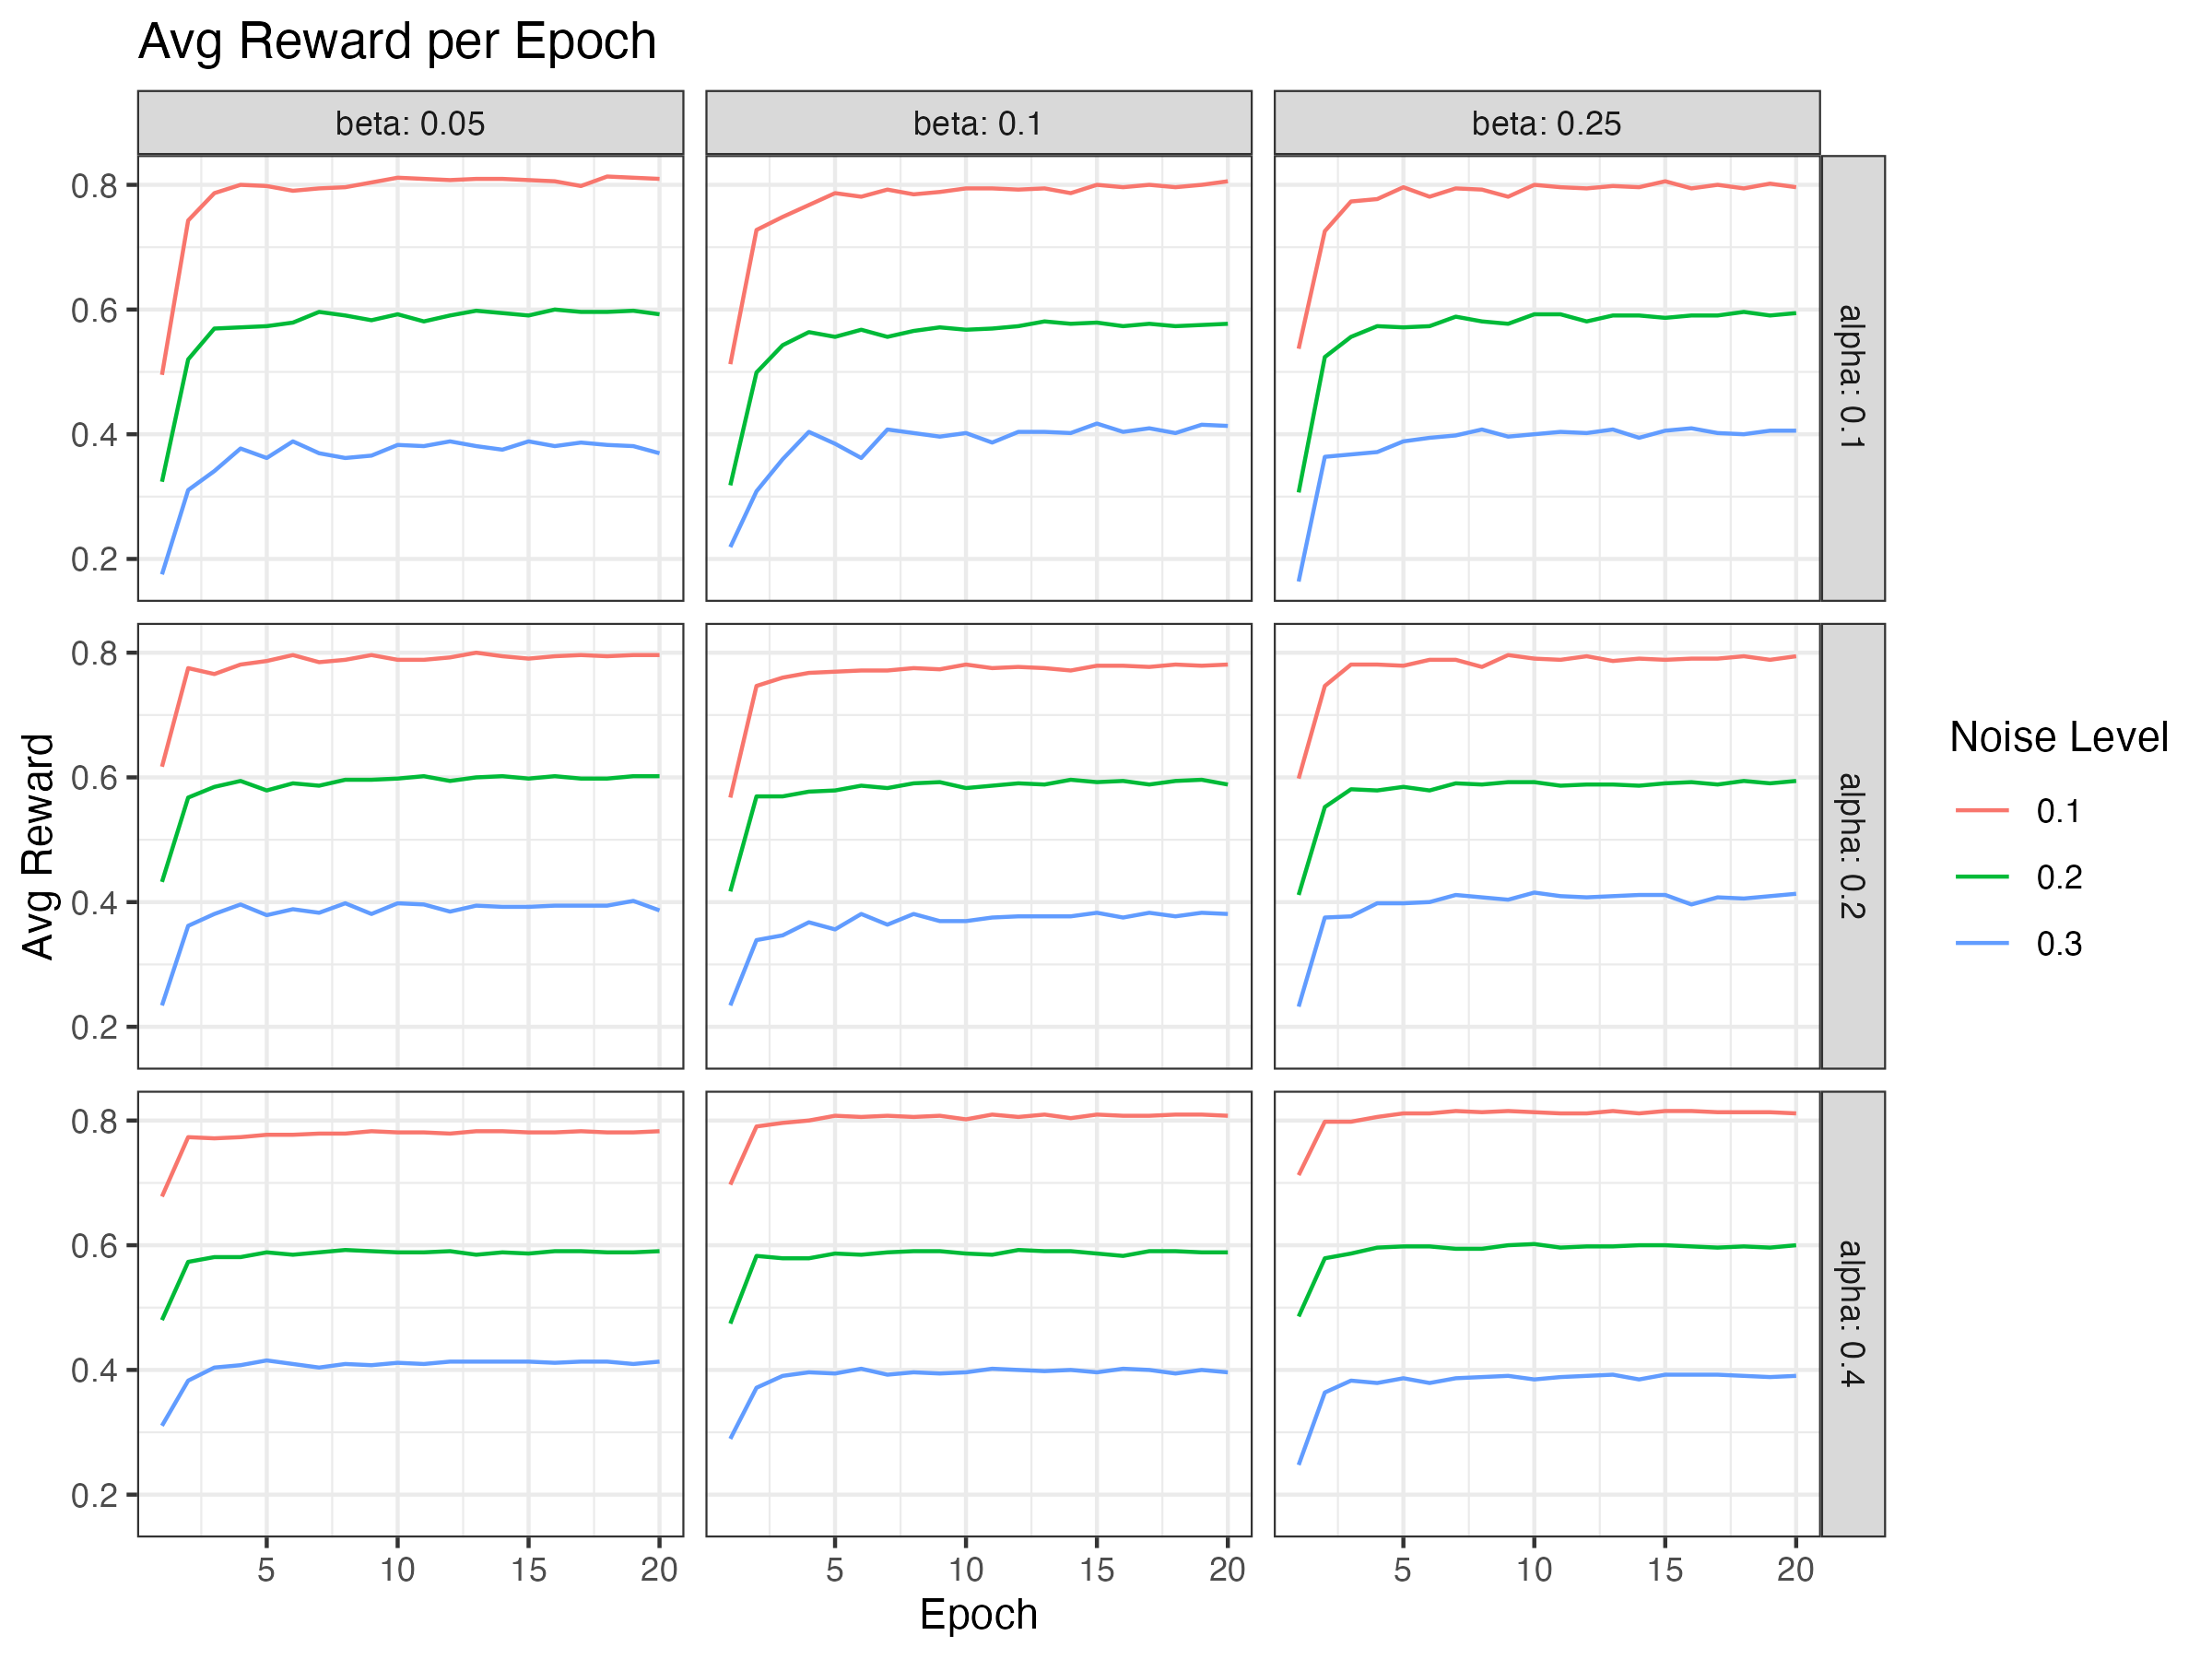
\includegraphics[width=0.99\textwidth]{../figures/epoch_reward.png}
    \caption{Average Reward per Epoch. This plot illustrates the evolution of the average reward during training, highlighting the model's improving performance across different parameter settings and noise levels.}
    \label{fig:epoch_reward}
\end{figure}

\begin{figure}[h]
    \centering
    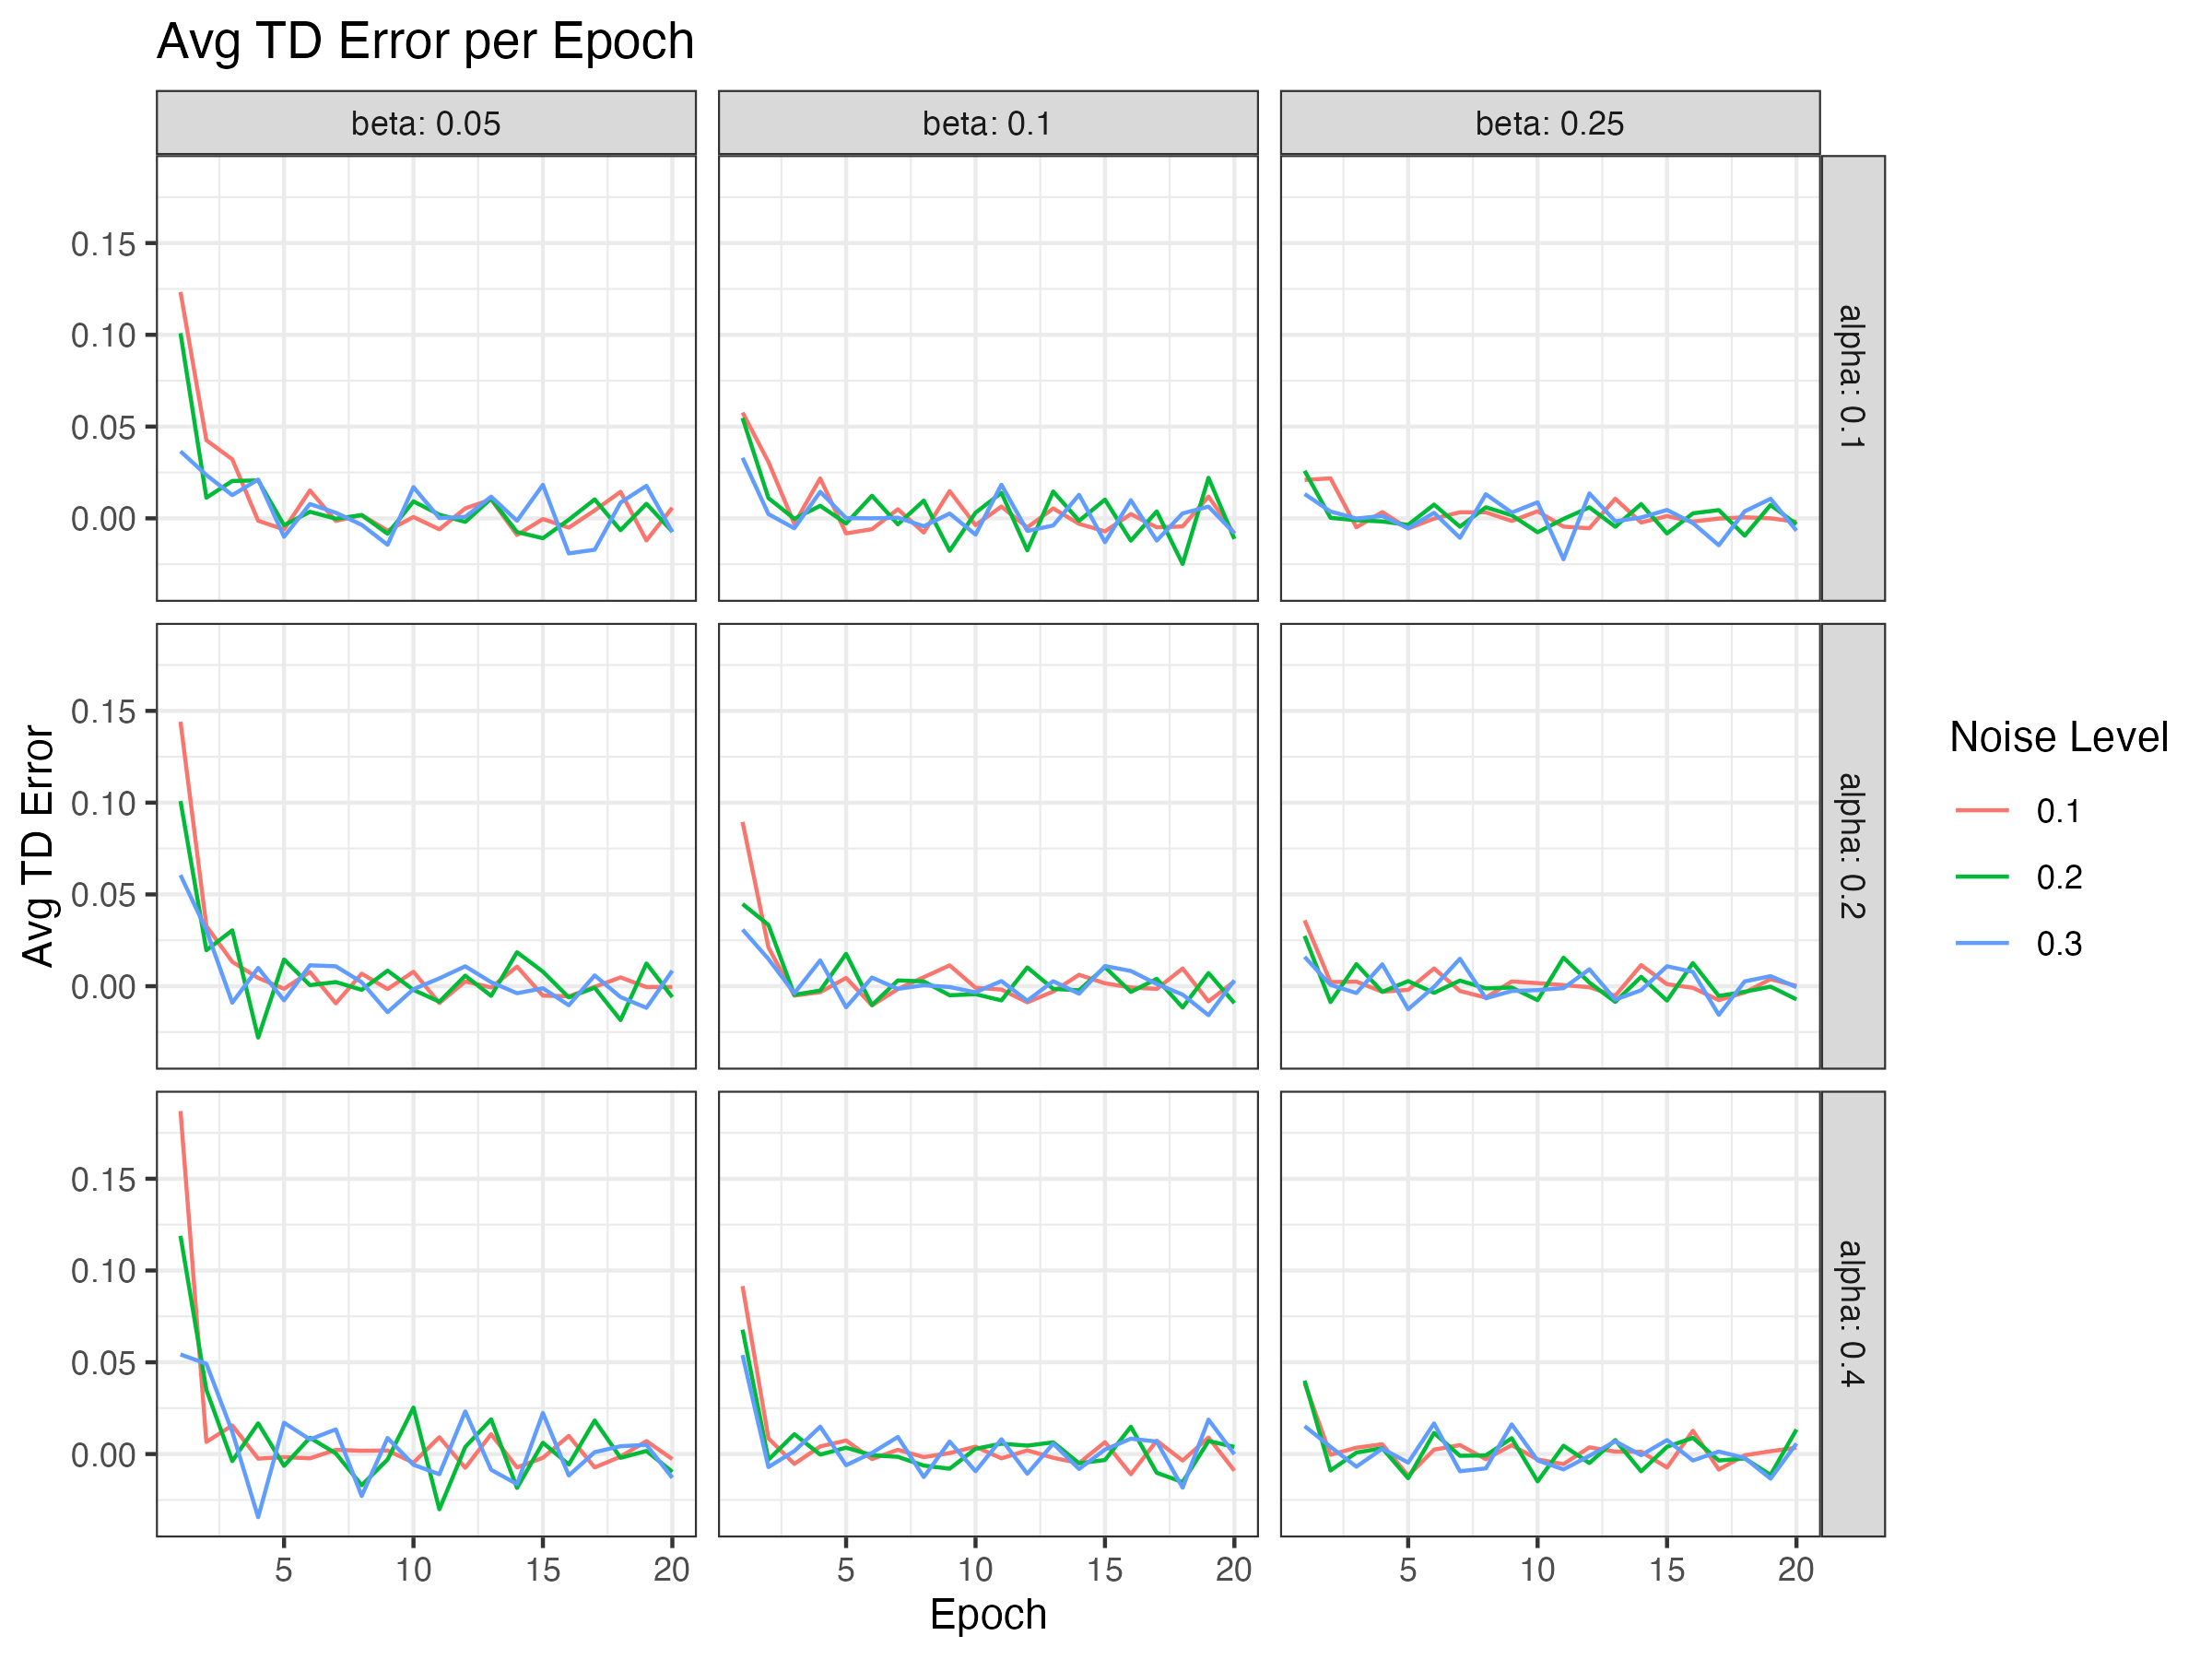
\includegraphics[width=0.99\textwidth]{../figures/epoch_td.png}
    \caption{Average Temporal-Difference (TD) Error per Epoch. This figure displays the convergence behaviour of the learning algorithm, with decreasing TD error over successive epochs indicating stabilisation of the value estimates.}
    \label{fig:epoch_td}
\end{figure}

\begin{figure}[h]
    \centering
    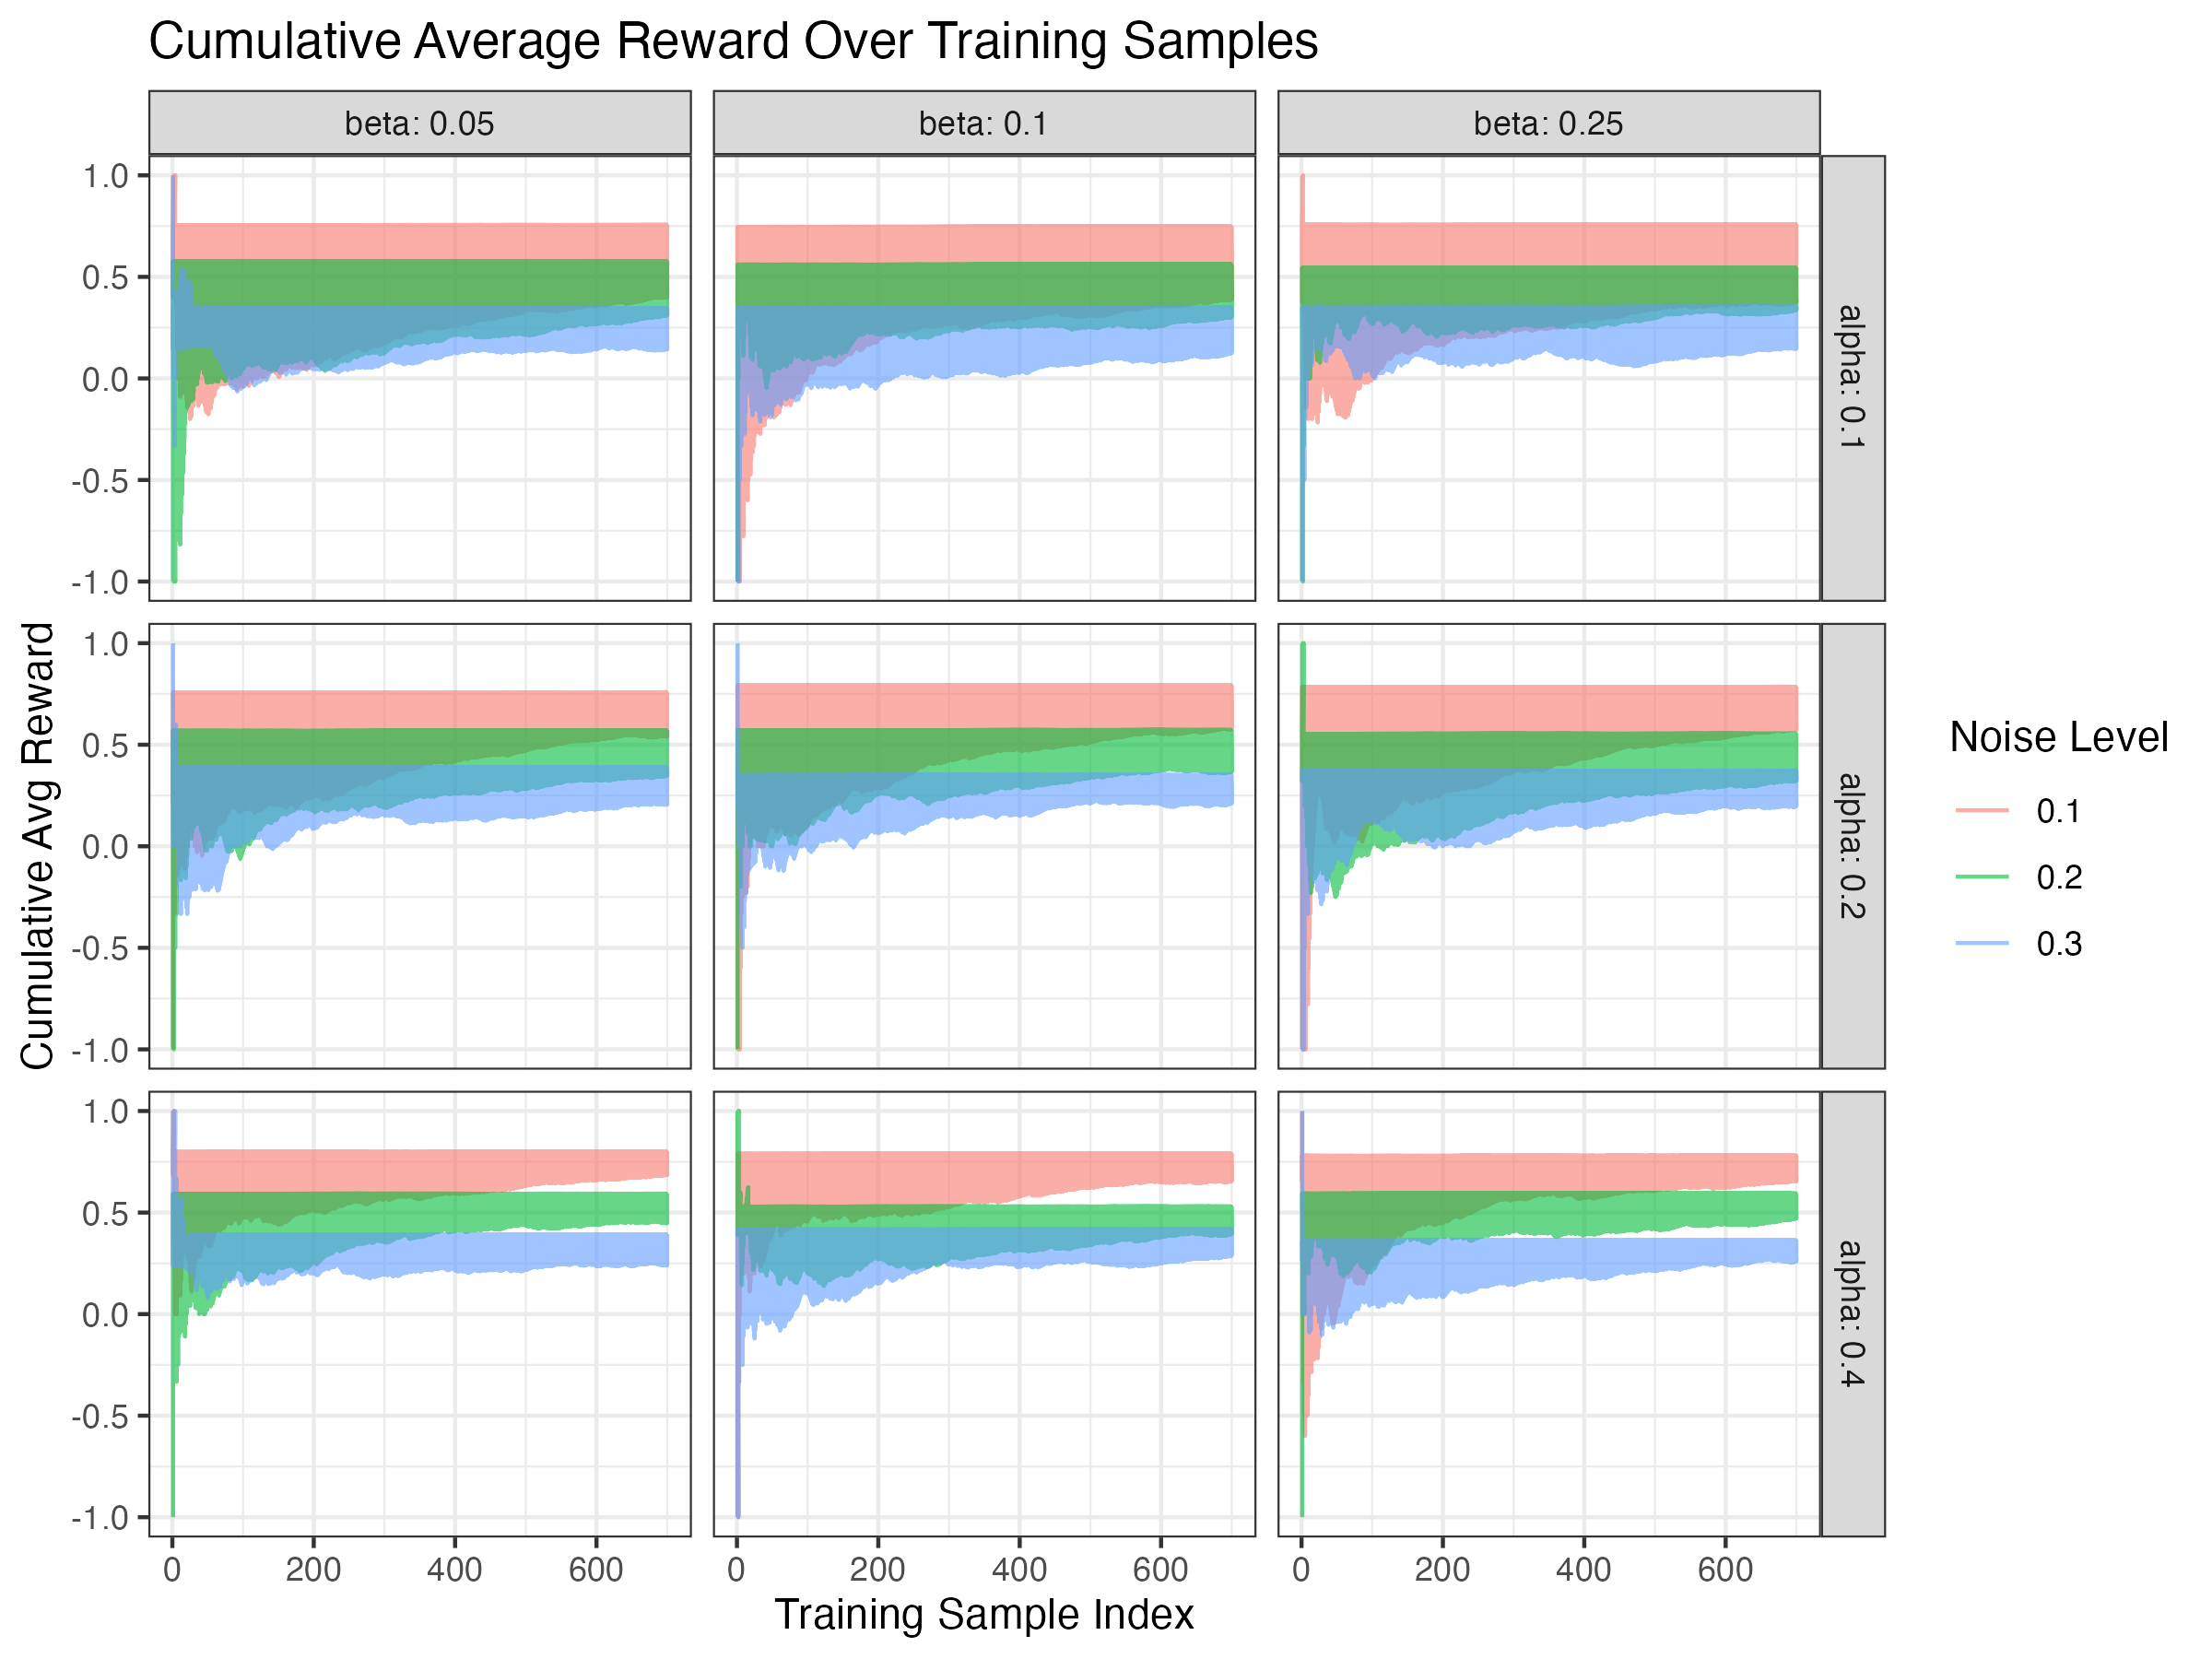
\includegraphics[width=0.99\textwidth]{../figures/learning.png}
    \caption{Cumulative Average Reward over Training Samples. The learning curve reflects the continuous improvement in model performance throughout training.}
    \label{fig:learning}
\end{figure}

\begin{figure}[h]
    \centering
    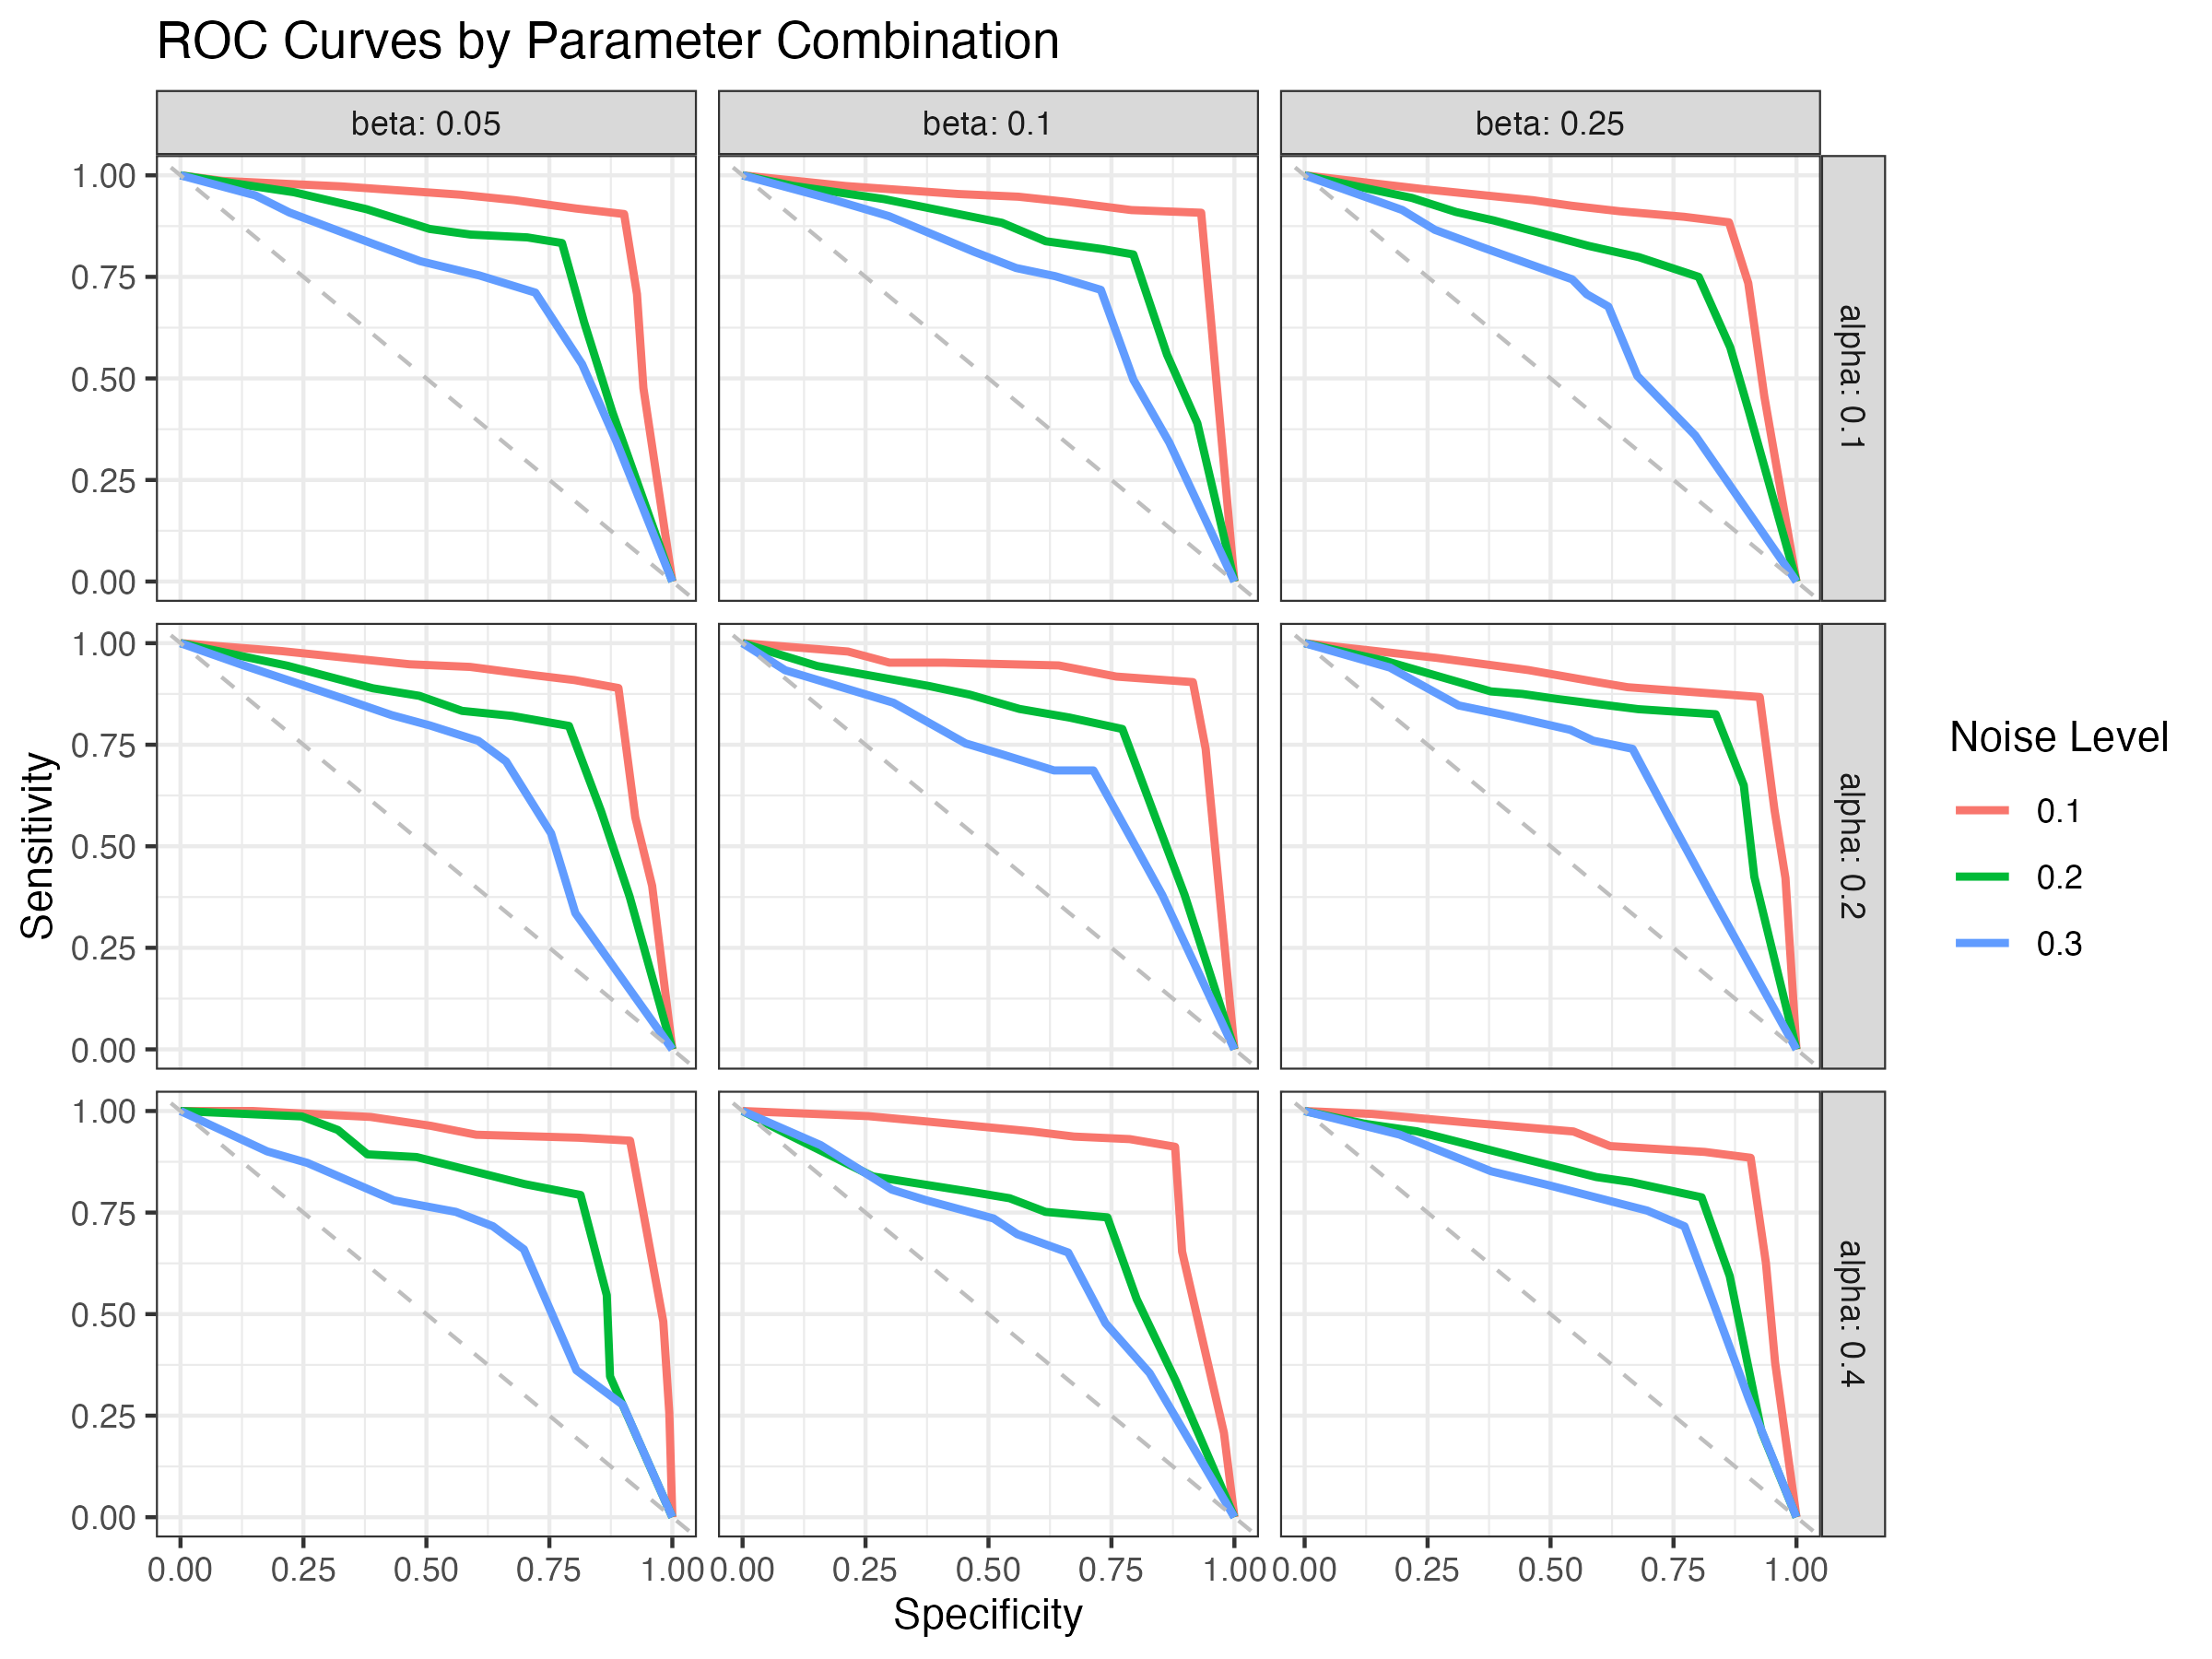
\includegraphics[width=0.99\textwidth]{../figures/roc_curve.png}
    \caption{Receiver Operating Characteristic (ROC) Curves by Parameter Combination. These curves illustrate the trade-off between the true positive and false positive rates, demonstrating high discrimination ability under certain parameter settings.}
    \label{fig:roc_curve}
\end{figure}

\begin{figure}[h]
    \centering
    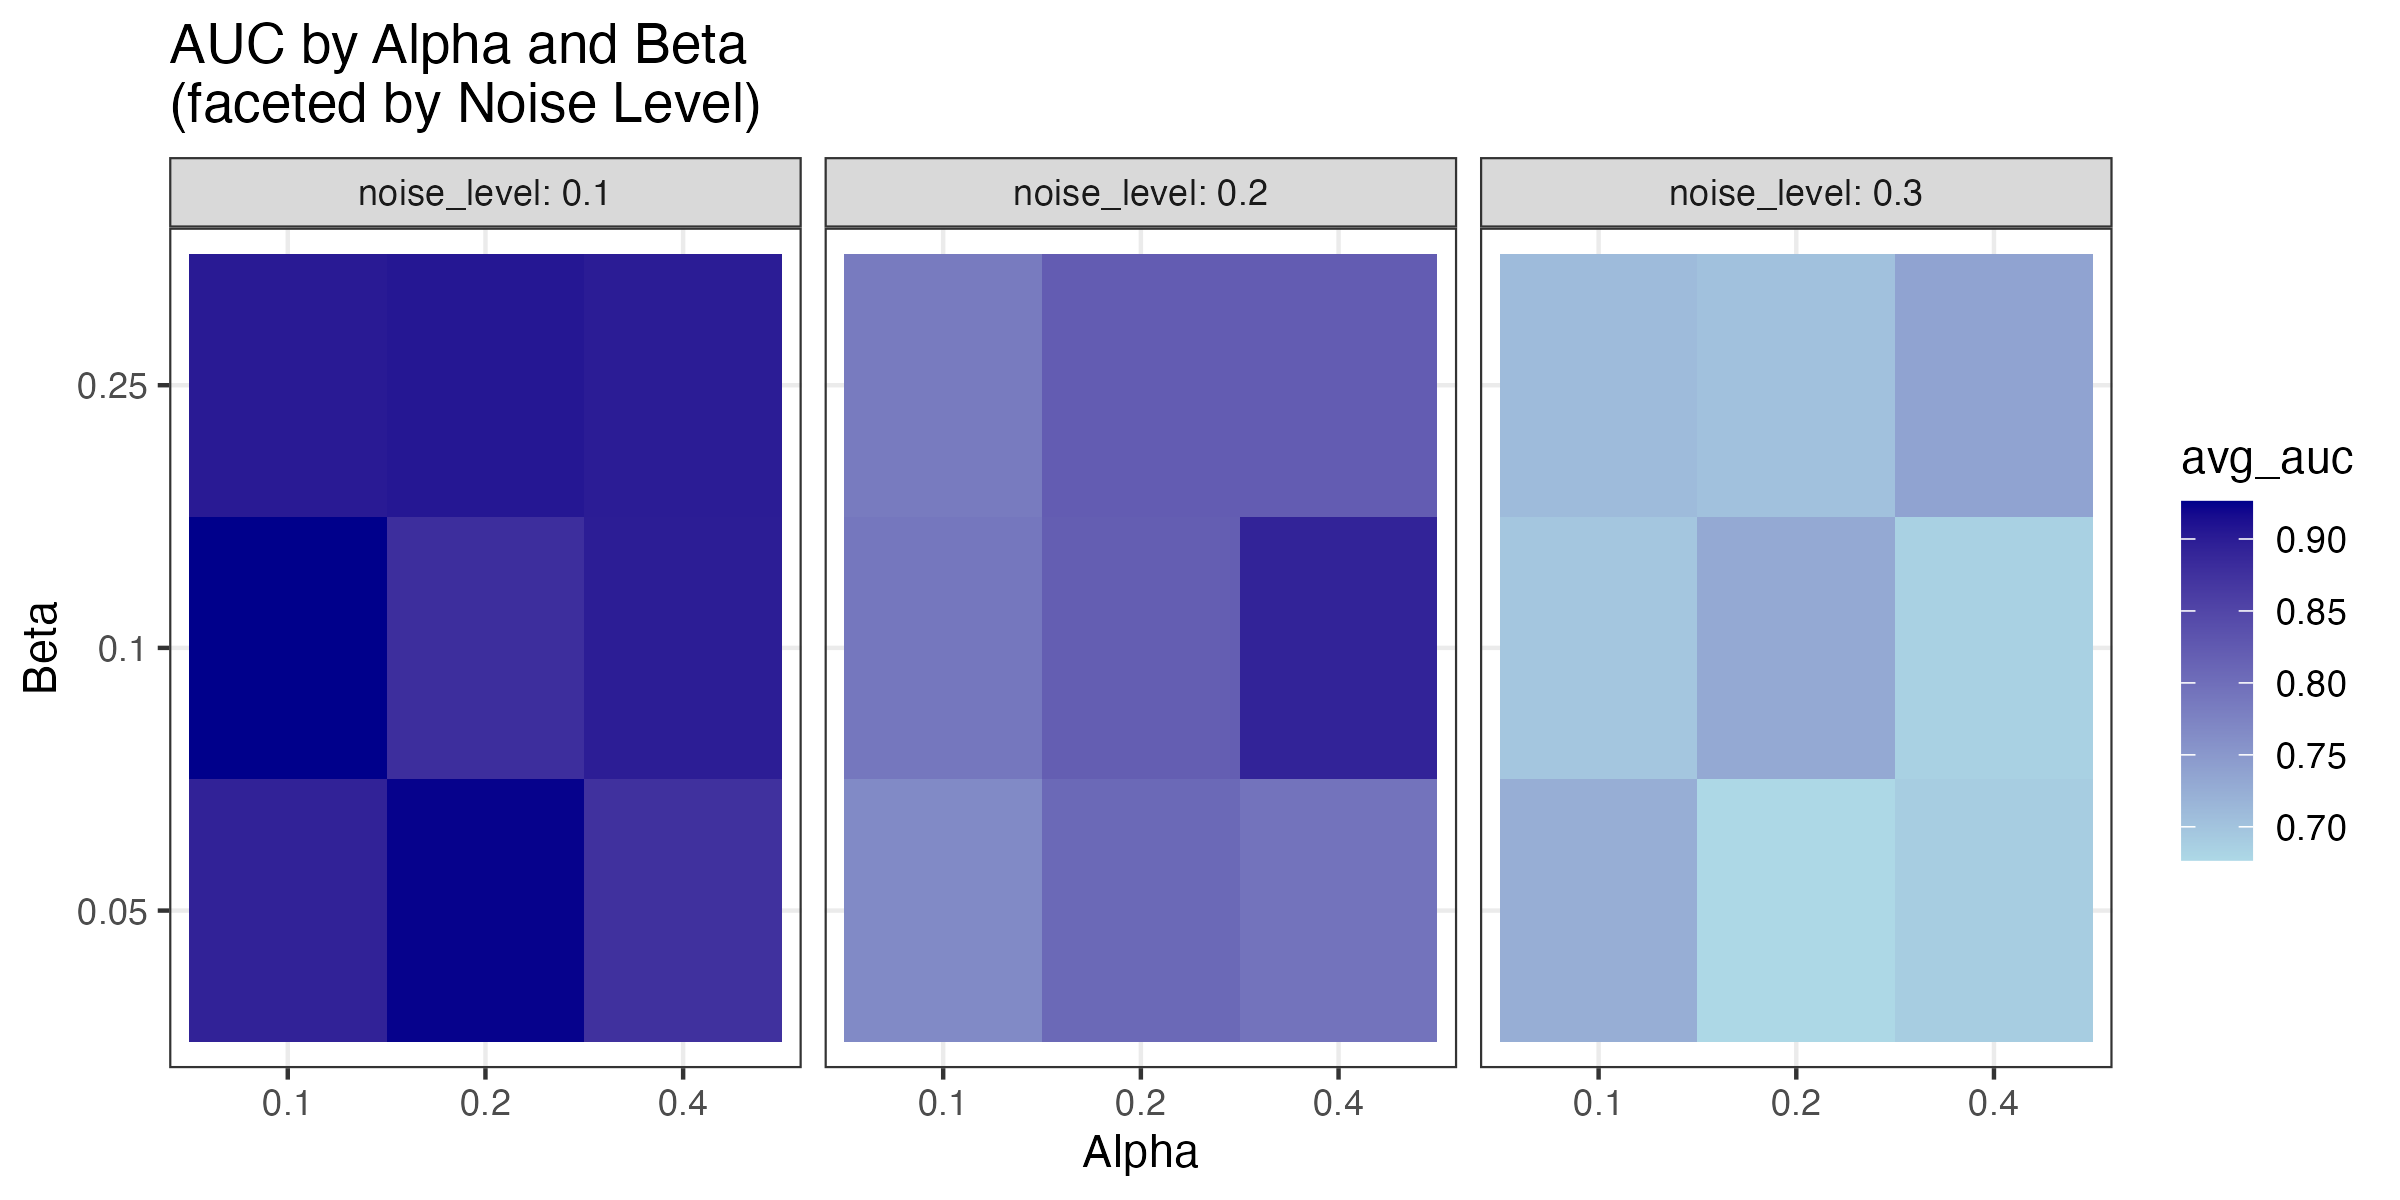
\includegraphics[width=0.99\textwidth]{../figures/auc.png}
    \caption{AUC Heatmap. This heatmap summarises the area under the ROC curve (AUC) as a function of the actor ($\alpha$) and critic ($\beta$) learning rates, faceted by noise level. Several combinations achieve AUC values exceeding 0.8, indicating robust classification performance.}
    \label{fig:auc}
\end{figure}

\begin{figure}[h]
    \centering
    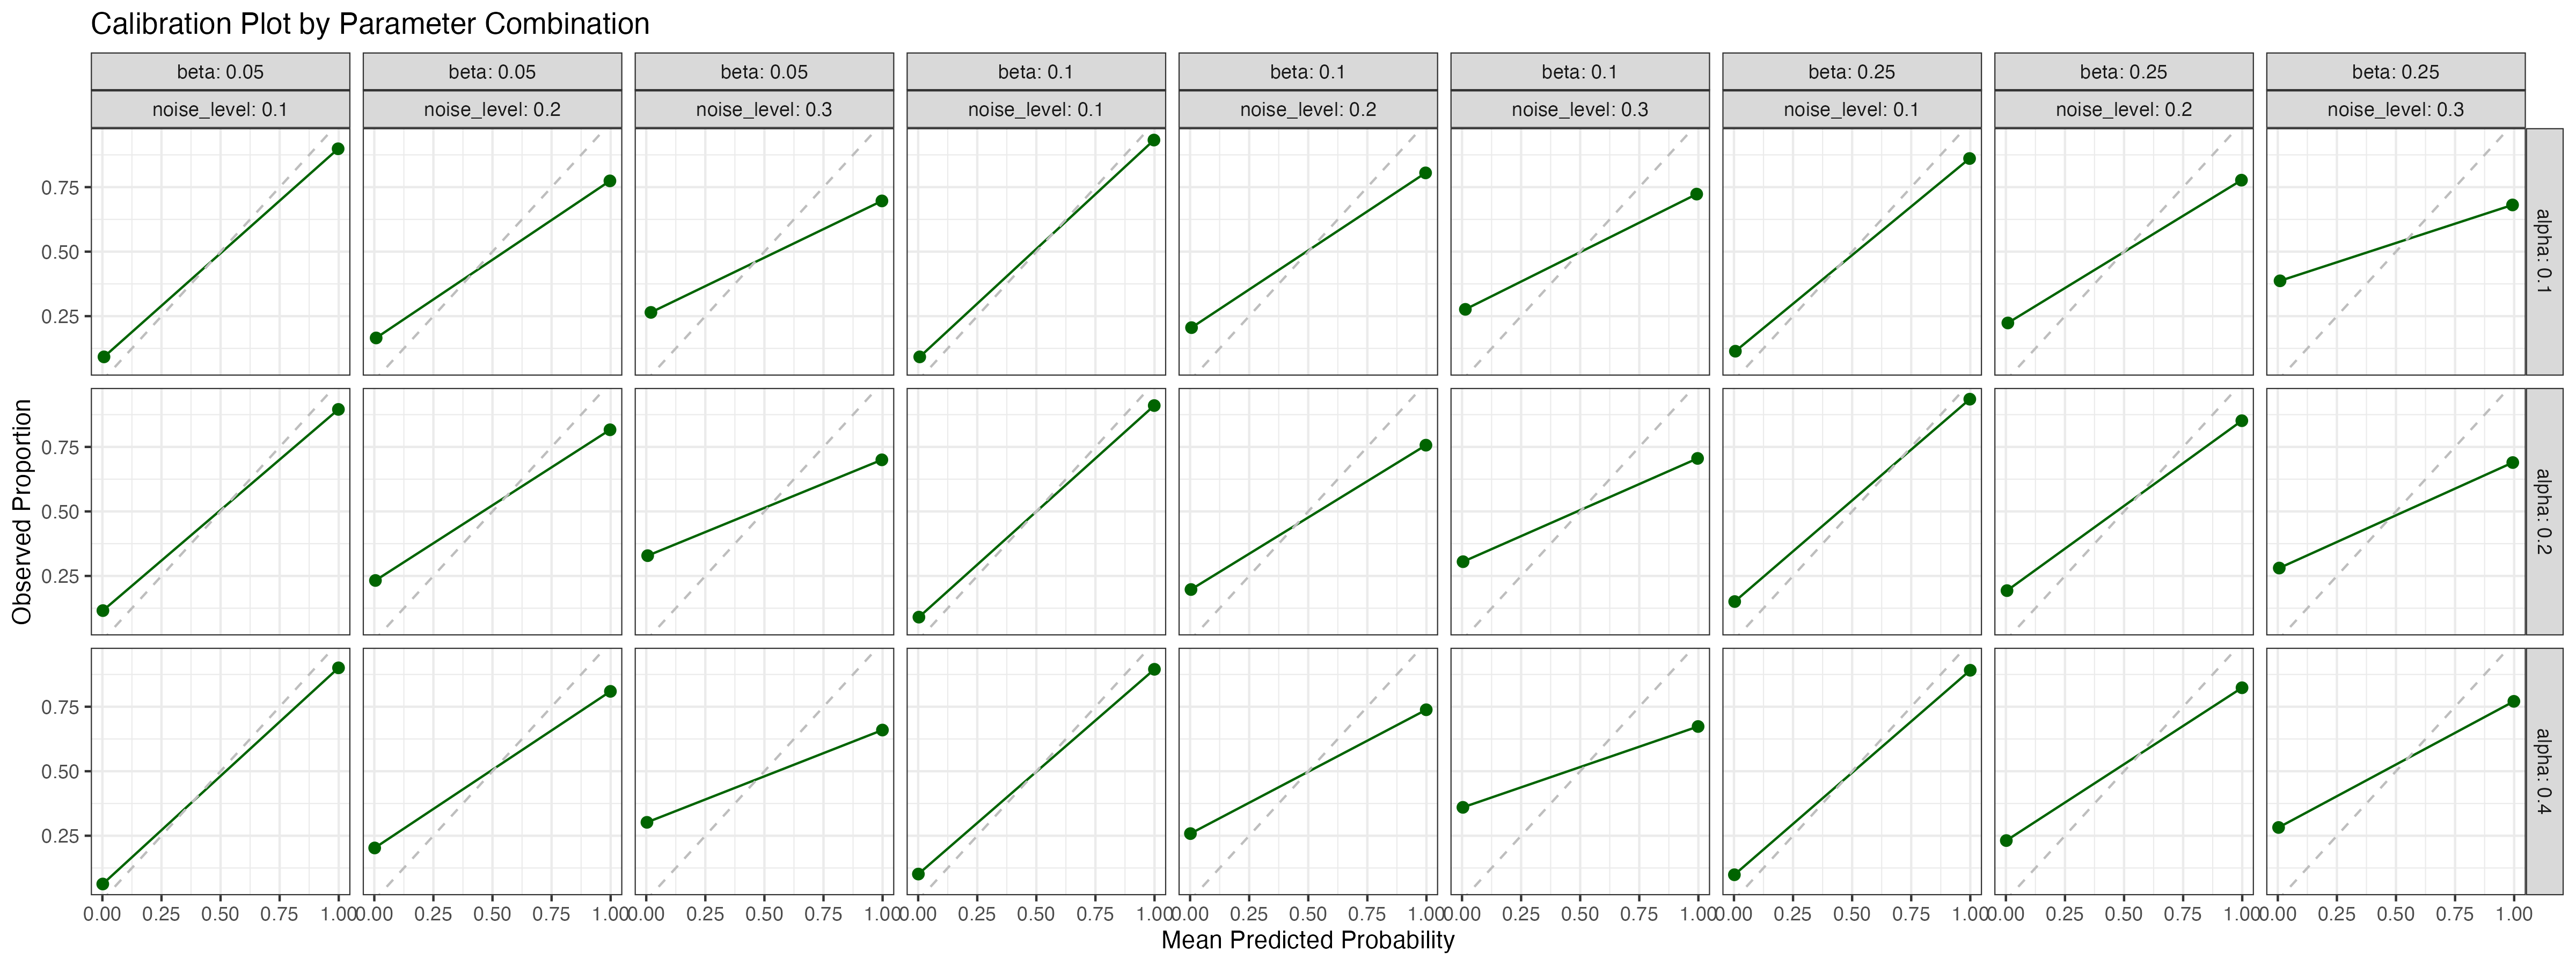
\includegraphics[width=0.99\textwidth]{../figures/calibration.png}
    \caption{Calibration Plot. This plot compares the mean predicted probabilities to the observed proportions of pathogenic variants, showing that the predicted probabilities are well-calibrated across various parameter combinations.}
    \label{fig:calibration}
\end{figure}


\clearpage

\section{Discussion}
In this study, we have established a reinforcement learning (RL) framework as an incremental step toward a broader Bayesian methodology aimed at classifying genetic variants for their pathogenic potential. Our current investigation focuses on evaluating RL methods on simulated data, explicitly quantifying multiple performance metrics relevant to the prediction of pathogenicity. By simulating scenarios reflective of real-world complexities, such as label noise and variant heterogeneity, we have elucidated which RL configurations exhibit robust and reliable performance.

The progressive improvement observed in average reward per epoch (Figure~\ref{fig:epoch_reward}) illustrates the model's capacity for effective learning despite varying levels of noise and different hyperparameter settings. Notably, the reduction in temporal-difference (TD) error across epochs (Figure~\ref{fig:epoch_td}) indicates successful convergence of our actor-critic RL algorithm. This stabilisation is critical, as it demonstrates the algorithm's ability to adaptively refine its predictions, which is a cornerstone for its utility in clinical genomic interpretation.

A critical aspect of reinforcement learning is its dynamic adaptability, which we have visualised clearly in the cumulative average reward curves (Figure~\ref{fig:learning}). This continuous upward trajectory highlights the model's ability to enhance predictive accuracy progressively throughout the training period. Such adaptability will be indispensable in practical genomic applications, where new variants continuously emerge, and datasets evolve.

Our analysis of ROC curves (Figure~\ref{fig:roc_curve}) and the corresponding heatmap of AUC values (Figure~\ref{fig:auc}) provides a comprehensive view of the predictive performance across varying parameters. Several parameter combinations produced robust discrimination performance, underscored by AUC values exceeding 0.8 even under challenging noise conditions. This finding emphasises the potential for selecting optimal RL hyperparameters tailored to specific genomic contexts and quality conditions in real datasets.

Calibration analysis (Figure~\ref{fig:calibration}) demonstrates that the RL model can generate accurate probability estimates that closely match observed pathogenic proportions. Reliable calibration is essential for clinical interpretation, as it provides confidence in the quantitative risk assessments derived from such models. The consistency observed across a variety of parameter settings strengthens the credibility of our RL-based predictions.

This study sets the stage for subsequent application of our RL framework to real genomic data, where the complexities encountered in simulations are amplified by biological variability and data imperfections. The current simulated environment has enabled us to systematically explore and quantify algorithm performance across controlled yet realistic scenarios. Our future work will focus on applying these RL methods to empirical genomic data, further integrating Bayesian frameworks to enhance interpretability, robustness, and clinical relevance.

Ultimately, this incremental methodological development has significant implications for the broader genomic research community. By refining predictive accuracy and interpretability, RL and subsequent Bayesian methodologies hold promise for transforming genetic diagnostics, enhancing clinical decision-making, and ultimately improving personalised healthcare.




\clearpage
\section{Conclusion}
We have presented an actor-critic reinforcement learning framework that leverages the GuRu score, gene number, and population frequency to predict the pathogenicity of genetic variants. By training on a dataset of known disease-causing variants and evaluating on unlabelled data, the model demonstrates promising performance across a range of parameter settings. The comprehensive evaluation, which includes ROC analysis, precision-recall metrics, learning curves and calibration assessments, highlights the potential of RL methodologies in the field of genetic diagnostics. This framework provides a solid foundation for further research into the integration of machine learning techniques with genomic data analysis and may ultimately contribute to improved personalised medical interventions.





\end{document}

\clearpage
\bibliographystyle{unsrtnat}
\bibliography{references}  



\end{document}
